\begin{tcolorbox}[colback=white!10!white,colframe=green!30!black,title=Nyquist] 
\begin{figure}[H]
    \begin{subfigure}{0.5\linewidth}
        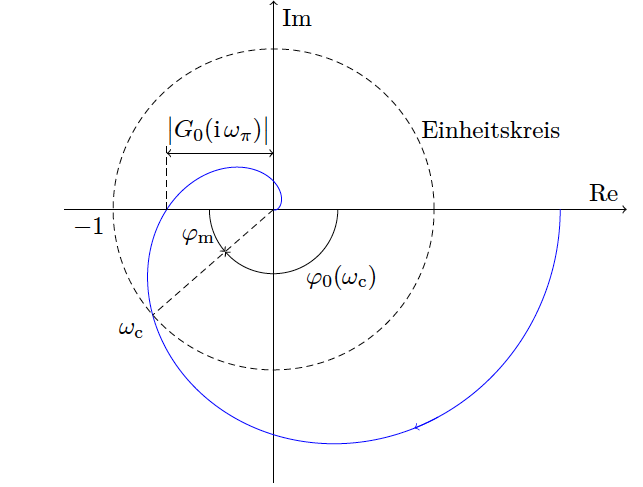
\includegraphics[width=\linewidth]{images/nyquist}
        \label{fig:nyquist}
    \end{subfigure}
    \begin{minipage}{0.45\linewidth}
        Amplituden-/ Betragsreserve 
        \begin{align*}
            &G_m = \frac{1}{|G_0(i\omega_\pi)|}\\
            & \omega_\pi = -180^{\circ}
        \end{align*}
        Phasenreserve ($\omega_c$ ist im Bode Diagramm, da wo Amplitudengang $0$dB schneidet):
        \begin{align*}
            &\phi_m = \pi + \phi(\omega_c)
        \end{align*}
        
    \end{minipage}
    Übliche Werte sind $G_m = 2,5 \ldots  10$ und $\phi_m = 30^{\circ} \dots 60^{\circ}  $. 
    
    Zur Stabilitätsanalyse kann man prüfen $|G_0(i\omega_\pi)| $ größer oder kleiner als 1 ist. 
\end{figure}
     \tcblower
     \begin{enumerate}
        \item Betrag und Phase für mehrere Punkte aus dem Amplitudengang und Phasengang des Bodediagramm ablesen. 
        \item Die Länge des Zeigers $10^{\frac{x}{20}}$ zum Nyquist-Plot ist der Wert im Amplitudengang.
        \item Der Winkel des Zeigers ist 
        \item Für $\omega = 0^{\circ}$ bis $\omega = \infty$
        \item Instabil, wenn derNyquist-Plot  die -1  umschließen.
     \end{enumerate}
     
 \begin{figure}[H]
     \begin{subfigure}{0.5\linewidth}
         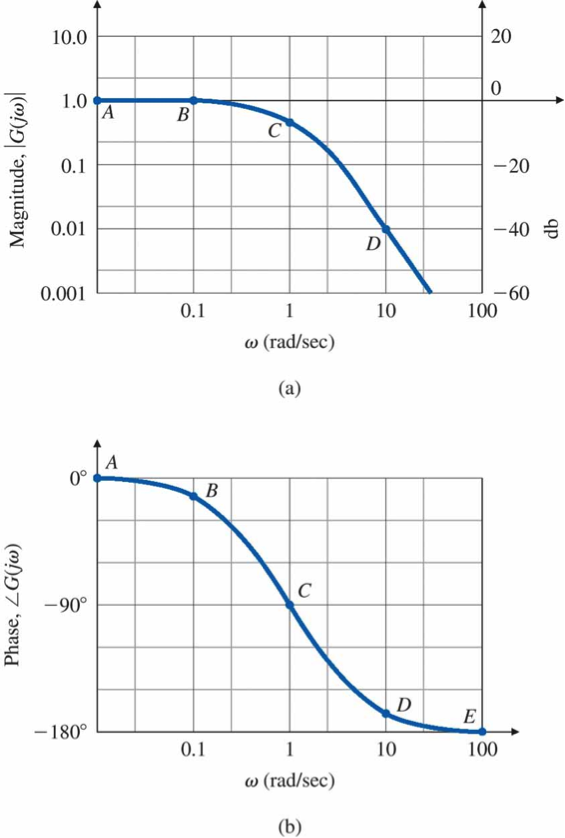
\includegraphics[width=\linewidth]{images/nyquist2}
     \end{subfigure}
     \begin{minipage}{0.45\linewidth}
         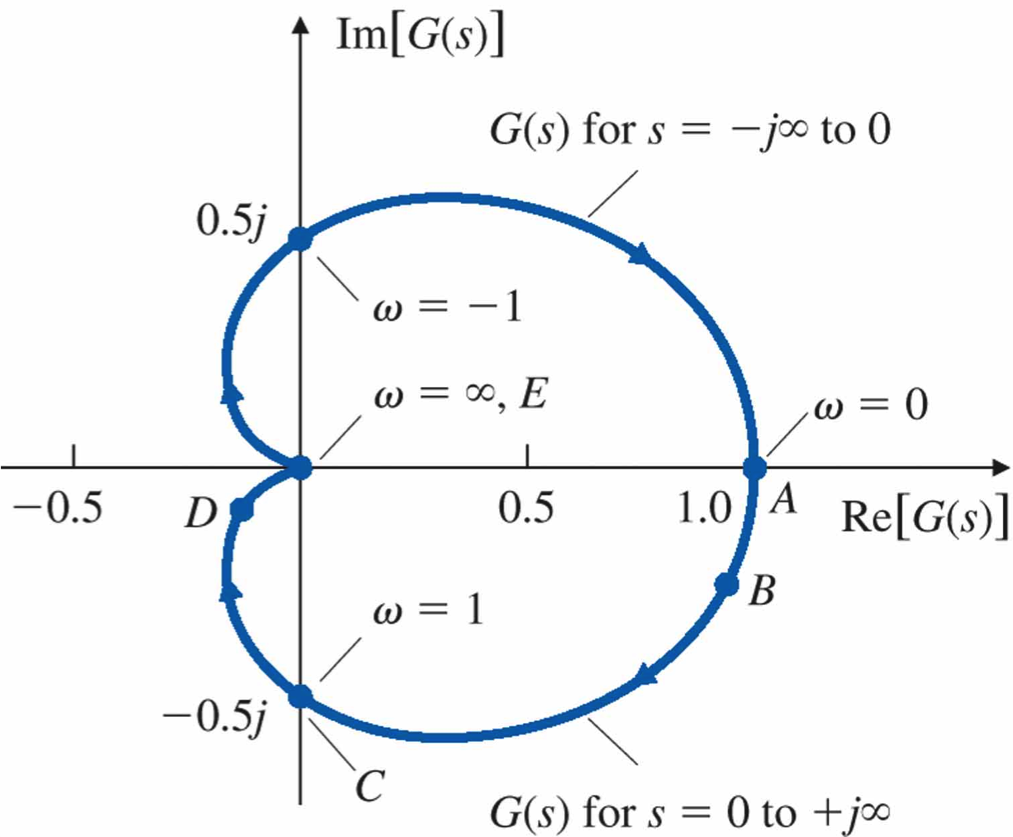
\includegraphics[width=\linewidth]{images/nyquist3}     
     \end{minipage}
 
 \end{figure}
\end{tcolorbox}

\begin{tcolorbox}[colback=white!10!white,colframe=red!60!black,title=Berechnung Betragsreserve aus G(s)]
     Gegeben ist eine Übertragungsfunktion:
     \begin{align*}
        &G(s) = \frac{10}{s^3+11s^2+11s+10}
     \end{align*}
     $j\omega$-Einsetzen  - und auf die untere Form bringen:
     
     Umformen auf
     \begin{align*}
         G(j\omega) &= \frac{10}{\text{Re} + j\omega \text{Im}} = \\
         &=\frac{10}{(-11\omega^2+10)+i\omega (11-\omega^2)}\\
         \tan(-\pi) &= 0 = \frac{\omega_{\pi}(11-\omega_{\pi}^2)}{ \omega_{\pi}^2 +10}\\
     \omega_{\pi} &= \sqrt{11}\\
     G(i\omega_{\pi}) &= \frac{10}{-111}  = 20,9 \text{dB}
     \end{align*}
     
    
\end{tcolorbox}
